\subsection{Vertex reconstruction}
In $pp$ collisions, where the charged-particle multiplicity is low, the vertex finding algorithm sometimes fails to find a primary vertex. In addition, at high luminosity, vertex finder can fail due to the contribution of pile-up events and providing a wrong reconstructed vertex. In this study we require at least two reconstructed global tracks $N^{global}_{reco}\geq 2$ passing all the quality cuts listed in Table \ref{tab:trackCut} but without $\textrm{DCA}_{xy}$ and $\textrm{DCA}_{z}$ cuts. 

\subsubsection{Track quality cuts used for vertexing}
A global track  used in vertex reconstruction has to pass the quality cuts listed in the Table \ref{tab:trackCutVertex}, which are different than used in the analysis. Since that, vertex reconstruction efficiency and fake vertex rate is calculated as a function of number of global tracks used in vertexing $N^{global}_{vrt}$ instead of $N^{global}_{reco}$. 


\begin{table}[H]
	\centering
	\begin{tabular}{| l | l |}
		\hline			
		Quantity & Cut \\
		\hline
		\hline
		Number of Fit Points & Fit Points $>20$\\
		Transverse Impact Parameter & $|d_0|<2$~cm\\ 
		Ratio of Fit Points / Possible Fit Points & Fit Points/ Possible Fit Points $>0.52$\\
		Global Track Transverse Momentum & $p_{T}>0.2$~GeV/c\\
		TOF Matched Track & TOF Match-Flag $\geq1$\\
		\hline  
	\end{tabular}
	\caption[Vertexing Track Level Cuts]{Vertexing Track Level Cuts}
	\label{tab:trackCutVertex}
\end{table}
\subsubsection{Vertex efficiency and fake vertex}
In every MC event there is a well defined primary vertex.  With the embedded
event reconstructed and the MC information in hand,
the vertex-finding efficiency can be obtained. In the analysis we require exactly one reconstructed vertex with at least two primary tracks passing the selection cuts $N_{reco}^{primary}\geq 2$. The vertex with the label \textit{best} is the one with the highest number of TOF-matched tracks. If there are more than one such vertices, the \textit{best} vertex is the one with the higher rank in the MuDst. The~following studies were done for events with the $z$-coordinate of the true-level primary vertex \mbox{$|V_z<80|$~cm}. The overall
vertex-finding efficiency, $\epsilon_{vrt}^ {best}\left(N_{vrt}^{global}\right)$, is determined as the
ratio of the number of good reconstructed events (reconstructed exactly one primary vertex with at least two primary TOF-matched tracks passing the quality cuts $N_{reco}^{primary}\geq 2$), with the reconstructed vertex matched to the true-level ptimary vertex, to the number of input MC events. The fake vertex
rate, $\delta_{vrt}^{fake}\left(N_{vrt}^{global}\right)$, is obtained as the ratio of the number 
of fake vertex events (exactly one reconstructed vertex, $N_{reco}^{primary}\geq 2$, but the reconstructed vertex not matched to the true-level primary vertex) to the number of input MC events. The vertex-finding efficiency and fake vertex rate as a function of $N^{global}_{vrt}$ is shown in  \Cref{fig:vertexingEffi,fig:vertexingFake}. Due to very large fake vertex rate $(>50\%)$ for events with many tracks, the main analysis was limited to events with $N_{reco}^{primary} < 8$ and $N_{reco}^{primary}<6$ for SD and CD, respectively. 
For events with exactly two global tracks used for vertexing, $N^{global}_{vrt}=2$, the vertex-finding efficiency and fake vertex rate were calculated as a function of the longitudinal distance between these tracks $|\Delta z_0|$, which is shown in \Cref{fig:vertexingEffiZ,fig:vertexingFakeZ}. The vertex-finding efficiency is smaller than $5\%$ for tracks with $|\Delta z_0|>2$~cm, hence the analysis was limited to the events with  $|\Delta z_0|<2$~cm, when $N^{global}_{vrt}=2$. Finally, each event is corrected for vertex-finding efficiency and fake vertex rate by the factor:
\begin{equation}
\frac{1}{\epsilon_{vrt}^ {best}\left(N_{vrt}^{global}\right) + \delta_{vrt}^{fake}\left(N_{vrt}^{global}\right)}
\label{eq:vertexEffi}
\end{equation}
\begin{figure}[h]
	\centering
	\parbox{0.484\textwidth}{
		\centering
		\begin{subfigure}[b]{\linewidth}{
				\subcaptionbox{\label{fig:vertexingEffi}}{\includegraphics[width=\linewidth, page=2]{graphics/vertexing/vertexEffi.pdf}}}
		\end{subfigure}
	}
	\quad
	\parbox{0.484\textwidth}{
		\centering
		\begin{subfigure}[b]{\linewidth}{
				\subcaptionbox{\label{fig:vertexingFake}}{\includegraphics[width=\linewidth, page=3]{graphics/vertexing/vertexEffi.pdf}}}
		\end{subfigure}
	}\\
	\parbox{0.484\textwidth}{
		\centering
		\begin{subfigure}[b]{\linewidth}{
				\subcaptionbox{\label{fig:vertexingEffiZ}}{\includegraphics[width=\linewidth, page=20]{graphics/vertexing/vertexEffi.pdf}}}
		\end{subfigure}
	}
	\quad
	\parbox{0.484\textwidth}{
		\centering
		\begin{subfigure}[b]{\linewidth}{
				\subcaptionbox{\label{fig:vertexingFakeZ}}{\includegraphics[width=\linewidth, page=21]{graphics/vertexing/vertexEffi.pdf}}}
		\end{subfigure}
	}
	\caption[Vertex-finding efficiency and fake vertex rate]{Vertex-finding efficiency and fake vertex rate as a function of number of tracks used in vertexing $N^{global}_{vrt}$ (a-b). For events with exactly two global tracks used for vertexing, $N^{global}_{vrt}=2$, the vertex-finding efficiency and fake vertex rate were calculated as a function of $|\Delta z_0|$ (c-d).}
	\label{fig:vertexEfficiency}
\end{figure}
\subsubsection{Fake vertex events}
From the MC study, the particle spectra from fake
vertex events are extracted and compared to those from
good events (with a correctly reconstructed vertex). It
is found that particles from the fake vertex events have
somewhat harder $p_T$ spectra than those in good events,
presumably due to the wrongly assigned reconstructed vertex to true-level primary vertex in final track fitting and the fact that higher $p_T$
particles are assigned larger weight in the vertex-fitting
algorithm. Figure \ref{fig:fakeVertexEvents} shows the ratio of the charged
hadron $p_T$ spectrum in good vertex events to that in all
events with a reconstructed vertex (i.e. sum of good and
fake vertex events) for SD~(a) and CD~(b).
The spectra are normalized per event before the
ratio is taken. This ratio is parameterized, and the parameterization,
$\epsilon_{fake}(p_T)$, is multiplied with all $p_T$ spectra
to correct for the $p_T$-dependent effect of the fake vertex
events. 
\begin{figure}[H]
	\centering
	\parbox{0.484\textwidth}{
		\centering
		\begin{subfigure}[b]{\linewidth}{
				{\includegraphics[width=\linewidth, page=19]{graphics/chargedMC/bkg0max.pdf}}}
		\end{subfigure}
	}
	\quad
	\parbox{0.484\textwidth}{
		\centering
		\begin{subfigure}[b]{\linewidth}{
				{\includegraphics[width=\linewidth, page=15]{graphics/chargedMC/bkg1max.pdf}}}
		\end{subfigure}
	}
	\caption[The $p_T$ dependent correction to particle spectra due
		to fake vertex events, $\epsilon_{fake}(p_T)$, in SD and CD collisions]{The $p_T$ dependent correction to particle spectra due
	to fake vertex events, $\epsilon_{fake}(p_T)$, in SD (a) and CD (b) collisions.}
	\label{fig:fakeVertexEvents}
\end{figure}
\subsubsection{Other corrections to the reconstructed vertices}
As it was mentioned in  the previous section, in the analysis only events with exactly one primary vertex. The~data was corrected for vetoing the events due to additional vertices reconstructed as a primary vertices:
\begin{enumerate}[label=(\alph*)]
\item more than one additional vertices
\item secondary vertex from the interactions with the dead material
\item fake vertex
\item primary vertex (vertex splitting or background vertex reconstructed as best vertex) 
\item decay vertex.  
\end{enumerate}
The correction was obtained as a ratio of the number of events with reconstructed best vertex
and additional fake/secondary vertices to all events with reconstructed best vertex as a function of $N^{global}_{vrt}$. As before, for events with $N^{global}_{vrt}=2$, the correction was calculated as a function of $|\Delta z_0|$. In the end, additional term was added to the factor from the Eq.~\ref{eq:vertexEffi}, which is used for correcting each event: 
\begin{equation}
\frac{1}{\epsilon_{vrt}^ {best}\left(N_{vrt}^{global}\right) + \delta_{vrt}^{fake}\left(N_{vrt}^{global}\right)}\cdot\frac{1}{1-a-b-c-d-e}
\end{equation}
where $a-e$ is the fraction of events with additional vertices (labels listed above) shown in \Cref{fig:vertexAdditional,fig:vertexAdditionalZ}.
\begin{figure}[H]
	\centering
	\parbox{0.3\textwidth}{
		\centering
		\begin{subfigure}[b]{\linewidth}{
				{\includegraphics[width=\linewidth, page=4]{graphics/vertexing/vertexEffi.pdf}}}
		\end{subfigure}
	}
	\quad
	\parbox{0.3\textwidth}{
		\centering
		\begin{subfigure}[b]{\linewidth}{
				{\includegraphics[width=\linewidth, page=7]{graphics/vertexing/vertexEffi.pdf}}}
		\end{subfigure}
	}
	\parbox{0.3\textwidth}{
		\centering
		\begin{subfigure}[b]{\linewidth}{
				{\includegraphics[width=\linewidth, page=10]{graphics/vertexing/vertexEffi.pdf}}}
		\end{subfigure}
	}
	\quad
	\parbox{0.3\textwidth}{
		\centering
		\begin{subfigure}[b]{\linewidth}{
				{\includegraphics[width=\linewidth, page=13]{graphics/vertexing/vertexEffi.pdf}}}
		\end{subfigure}
	}
	\parbox{0.3\textwidth}{
			\centering
			\begin{subfigure}[b]{\linewidth}{
					{\includegraphics[width=\linewidth, page=16]{graphics/vertexing/vertexEffi.pdf}}}
			\end{subfigure}
		}
	\caption[Fraction of events with reconstructed best vertex and additional reconstructed vertices  as a function of $N_{vrt}^{global}$]{Fraction of events with reconstructed best vertex and additional reconstructed vertices as a function of $N_{vrt}^{global}$: more than one additional vertices (a), additional vertex from the interactions with dead material (b), additional fake vertex (c), additional primary vertex (d), additional decay vertex (e).}
	\label{fig:vertexAdditional}
\end{figure}
\begin{figure}[H]
	\centering
	\parbox{0.3\textwidth}{
		\centering
		\begin{subfigure}[b]{\linewidth}{
				{\includegraphics[width=\linewidth, page=22]{graphics/vertexing/vertexEffi.pdf}}}
		\end{subfigure}
	}
	\quad
	\parbox{0.3\textwidth}{
		\centering
		\begin{subfigure}[b]{\linewidth}{
				{\includegraphics[width=\linewidth, page=25]{graphics/vertexing/vertexEffi.pdf}}}
		\end{subfigure}
	}
	\parbox{0.3\textwidth}{
		\centering
		\begin{subfigure}[b]{\linewidth}{
				{\includegraphics[width=\linewidth, page=28]{graphics/vertexing/vertexEffi.pdf}}}
		\end{subfigure}
	}
	\quad
	\parbox{0.3\textwidth}{
		\centering
		\begin{subfigure}[b]{\linewidth}{
				{\includegraphics[width=\linewidth, page=31]{graphics/vertexing/vertexEffi.pdf}}}
		\end{subfigure}
	}
	\parbox{0.3\textwidth}{
			\centering
			\begin{subfigure}[b]{\linewidth}{
					{\includegraphics[width=\linewidth, page=34]{graphics/vertexing/vertexEffi.pdf}}}
			\end{subfigure}
		}
	\caption[Fraction of events with reconstructed best vertex and additional reconstructed vertices  as a function of $|\Delta z_0|$]{Fraction of events with reconstructed best vertex and additional reconstructed vertices as a function of $|\Delta z_0|$: more than one additional vertices (a), additional vertex from the interactions with dead material (b), additional fake vertex (c), additional primary vertex (d), additional decay vertex (e).}
	\label{fig:vertexAdditionalZ}
\end{figure}